% Chapter 1
\chapter{مقدمه}

\section{شناخت موضوع}
در سال‌های اخیر، پیشرفت‌های سریع فناوری و دسترسی آسان به اینترنت باعث شده‌اند که بسیاری از دستگاه‌های اطراف ما به اینترنت متصل شوند. این پدیده که به اینترنت اشیا%
\LTRfootnote{Internet of Things}
معروف است، شامل انواع دستگاه‌ها از جمله دستگاه‌های پوشیدنی%
\LTRfootnote{Wearable Devices}%
، خودروهای خودران، خانه‌های هوشمند%
\LTRfootnote{Smart Homes}
و به ویژه تلفن‌های هوشمند%
\LTRfootnote{Smart Phones}
می‌شود. این دستگاه‌ها به طور چشمگیری زندگی روزمره انسان‌ها را دگرگون کرده‌اند. استفاده از این سیستم‌ها همگی باعث تولید حجم قابل توجهی داده در طول روز می‌شوند که شرکت‌های بزرگ فناوری از این داده‌ها بهره برده و با استفاده از آن‌ها اقدام به انواع سرویس‌‌دهی به کاربران خود می‌نمایند.

با پیشرفت علم هوش مصنوعی و استفاده گسترده از روش‌های یادگیری ماشین، امکان بهره‌برداری بهینه از حجم عظیم داده‌های تولید شده فراهم شده است. این داده‌ها می‌توانند برای اجرای الگوریتم‌های مختلف به منظور دستیابی به اهداف متنوع به کار گرفته شوند. روش‌های متعددی برای مدیریت و اجرای این الگوریتم‌های یادگیری وجود دارد که در ادامه به توضیح هر یک پرداخته خواهد شد.


\subsection{یادگیری متمرکز}
روش یادگیری متمرکز%
\LTRfootnote{Centralized Learning}
که در بسیاری از سیستم‌های امروزی به کار می‌رود، به این صورت عمل می‌کند که تمامی گره‌ها%
\LTRfootnote{Nodes}
اطلاعات خود را به صورت کامل به سرویس‌دهنده ابری%
\LTRfootnote{Cloud Server}
ارسال می‌کنند. سرویس‌دهنده ابری با دسترسی به تمامی داده‌ها، الگوریتم‌های مورد نظر را اجرا می‌کند
\cite{elbir2022family}.
این روش در شکل
\ref{centralized_decentralized_learning}%
(الف) به تصویر کشیده شده است.


\subsection{یادگیری غیر متمرکز}
در روش یادگیری غیر متمرکز%
\LTRfootnote{Decentralized Learning}
، هر گره به صورت مستقل الگوریتم‌های مورد نظر را اجرا می‌کند. پس از چند مرحله اجرای کد، اطلاعات به‌روز شده را با گره‌های همسایه به اشتراک می‌گذارد. این فرآیند تا زمانی ادامه می‌یابد که تمامی گره‌ها به یک مقدار مشخص همگرا شوند
\cite{zhou2019edge}.
این روش در شکل
\ref{centralized_decentralized_learning}%
(ب) نشان داده شده است.

\begin{figure}[b]
	\centering
	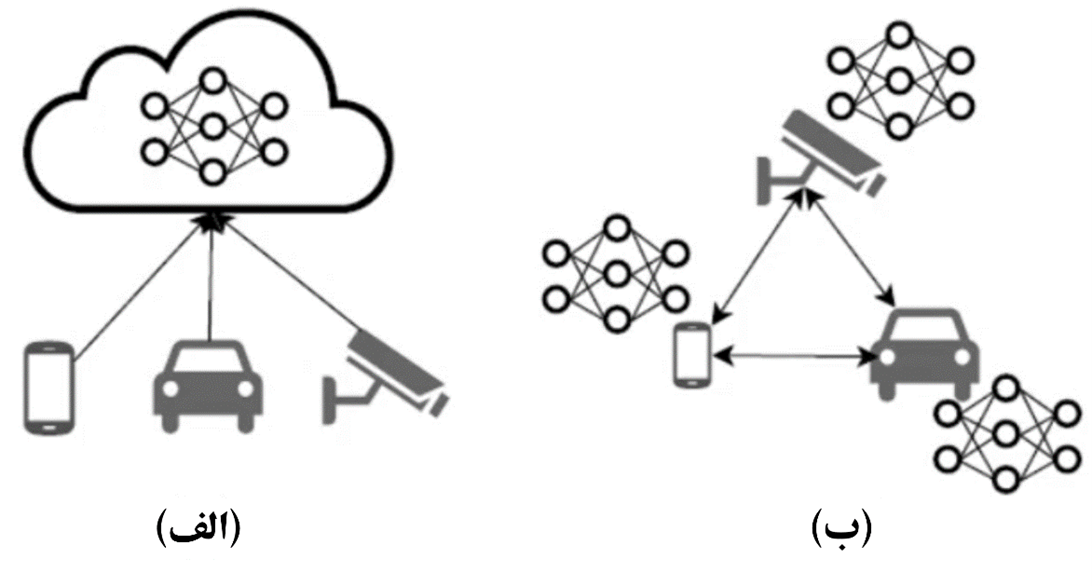
\includegraphics[scale=0.8]{images/chap1/centralized_decentralized_learning.png}%
	\caption{%
		(الف) یادگیری متمرکز، (ب) یادگیری غیرمتمرکز
		\cite{zhou2019edge}%
		.
	}
	\label{centralized_decentralized_learning}
	\centering
\end{figure}


\subsection{یادگیری توزیع شده}
در روش یادگیری توزیع‌شده%
\LTRfootnote{Distributed Learning}
، یک هسته مرکزی مسئولیت مدیریت کل سیستم و تمامی داده‌ها را بر عهده دارد. با این حال، به دلیل نیاز به توان پردازشی بالا، این هسته بار پردازشی را بین گره‌های موجود تقسیم می‌کند. در این رویکرد، فرض بر این است که تمامی گره‌ها دارای توان پردازشی یکسانی هستند و داده‌ها به طور مساوی بین گره‌ها توزیع می‌شوند. این روش در شکل
\ref{distributed_learning}
نشان داده شده است.


\begin{figure}[t]
	\centering
	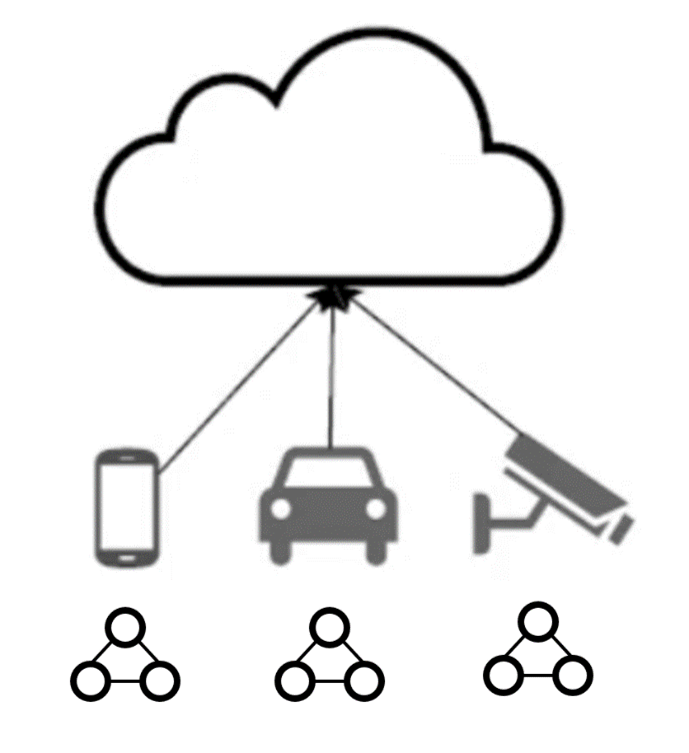
\includegraphics[scale=0.35]{images/chap1/distributed_learning.png}%
	\caption{%
		یادگیری توزیع شده.
		%		\cite{zhou2019edge}%
	}
	\label{distributed_learning}
	\centering
\end{figure}

\section{یادگیری فدرال}
سیستم‌های متمرکز تا پیش از این بیشتر نیازها را برطرف می‌کردند، اما در دنیای امروزی و با افزایش تعداد دستگاه‌های متصل، چالش‌های جدیدی مطرح شده است. هزینه‌های بالای مرتبط با انتقال حجم زیاد داده‌ها از یک جهت، و افزایش نگرانی‌ها درباره امنیت اطلاعات حساس و شخصی از جهت دیگر، محققان را به سمت استفاده از الگوریتم‌های غیرمتمرکز و توزیع‌شده در حوزه یادگیری ماشین سوق داده است. یکی از جدیدترین زیرمجموعه‌های مهم و پرکاربرد روش‌های یادگیری توزیع‌شده، یادگیری فدرال است که بسیار مورد توجه قرار گرفته است.


در روش یادگیری فدرال، برخلاف رویکردهای متمرکز یادگیری ماشین، تجزیه و تحلیل داده‌ها به دستگاه‌های لبه%
\LTRfootnote{Edge Devices}
یا سرویس‌گیرنده‌ها%
\LTRfootnote{Clients}
منتقل می‌شود. این روش، به عنوان یک جایگزین مطلوب برای مدل‌سازی داده‌ها در محیط‌هایی با تعداد زیادی سرویس‌گیرنده معرفی شده است. در این چارچوب، به جای انتقال داده‌های اصلی، پارامترهای مدل‌های محلی در هر مرحله از فرآیند آموزش به سمت سرور منتقل می‌شوند، که این امر توانایی بهبود امنیت و کاهش هزینه‌های ارتباطی را فراهم می‌کند.
در شکل
\ref{federated_learning}
این معماری به نمایش گذاشته شده است.


 \begin{figure}[t]
	\centering
	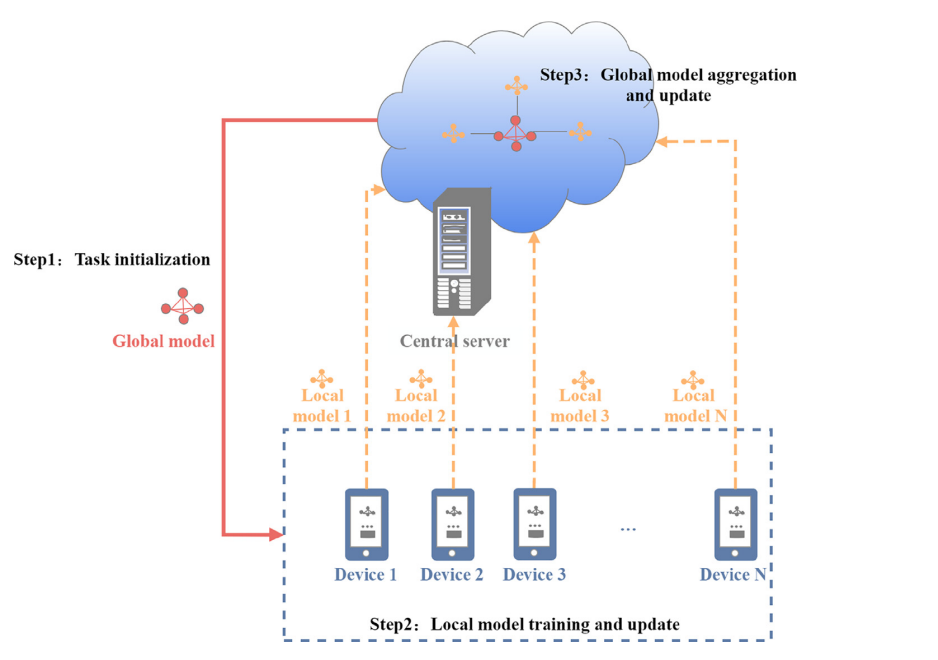
\includegraphics[scale=0.7]{images/chap1/federated_learning.png}%
	\caption{%
		یادگیری فدرال 
		\cite{ma2022state}%
		.
	}
	\label{federated_learning}
	\centering
\end{figure}

سرور در حقیقت نقش رهبری را ایفا می‌کند و با توجه به نوع داده‌ها، یک مدل شبکه عصبی%
\LTRfootnote{Neural Network}
ایجاد کرده و آن را به سمت کاربران ارسال می‌کند. در ادامه کاربران با توجه به داده‌های خود شبکه را آموزش می‌دهند و بعد از چند بار تکرار به صورت محلی، وزن‌های به‌روزرسانی شده را به سمت سرور بر می‌گردانند. همان‌طور که در شکل
\ref{federated_learning}
مشاهده می‌شود، داده‌ها همگی در سمت کاربران قرار گرفته‌اند و به سمت سرور ارسال نمی‌شوند. عدم اجبار در به اشتراک گذاشتن اطلاعات گره‌ها در یادگیری فدرال، کمک شایانی به حفظ حریم شخصی کاربران می‌کند
\cite{smith2017federated}.





% ابتدای فصل بهار سال 2017 محققین گوگل (Google) طی یک مطلب کوتاه در وبلاگ هوش مصنوعی، برای اولین بار موضـوع یادگیری فدرال را تحـت مطلبی با عنوان "یادگیری فدرال: یادگیری ماشین اشتـراکی، بدون آموزش متمرکز داده‌ها" مطرح نمودند. در این مطلب به طور کوتاه Google Keyboard یا به اختصار Gboard معرفی شد که با به کاری‌گیری یادگیری فدرال، لغت بعدی را پیش‌بینی و به کاربر توصیه می‌نمود. یادگیری فدرال در این کاربرد، نیاز به ارسال داده‌های کاربران به سمت سرور را حذف کرده است و به طور محلی مدل را به‌روزرسانی می‌کند.
%بنابراین، با بهره‌گیری از اطلاعات پنهان بسیار زیاد دستگاه‌ها در فرآیند مدل‌سازی، ضمن حفظ حریم شخصی سرویس‌گیرنده‌ها خدمات بهتری نسبت به قبل ارائه می‌گردد. در شکل نحوه استفاده از یادگیری فدرال در این برنامه به نمایش درآمده است.



\section{تاریخچه یادگیری فدرال}


در اوایل فصل بهار سال 2017، محققان گوگل
\lr{(Google)}
برای اولین بار موضوع یادگیری فدرال را در یک مطلب کوتاه در وبلاگ هوش مصنوعی خود معرفی کردند. این مطلب با عنوان "یادگیری فدرال: یادگیری ماشین اشتراکی، بدون نیاز به آموزش متمرکز داده‌ها" منتشر شد
\cite{mcmahan2017federated}.
در این نوشته، به طور مختصر از
\lr{Google Keyboard}
یا به اختصار
\lr{Gboard}
صحبت شد که با بهره‌گیری از یادگیری فدرال، قابلیت پیش‌بینی و پیشنهاد لغت بعدی به کاربر را دارد. با استفاده از یادگیری فدرال، دیگر نیازی به ارسال داده‌های کاربران به سرور نبود و مدل به ‌صورت محلی به‌روزرسانی می‌شد.

این روش، با بهره‌گیری از اطلاعات بسیار زیاد ذخیره شده در دستگاه‌ها، بدون نیاز به ارسال داده‌های حساس به سرور، به حفظ حریم شخصی کاربران کمک کرده و خدمات بهتری را ارائه می‌دهد. در شکل
\ref{gboard}%
، نحوه استفاده از یادگیری فدرال در این برنامه به نمایش درآمده است.


%در ابتدای فصل بهار سال 2017 محققین گوگل
%\lr{(Google)}
%طی یک مطلب کوتاه در وبلاگ هوش مصنوعی، برای اولین بار موضـوع یادگیری فدرال را تحـت مطلبی با عنوان "یادگیری فدرال: یادگیری ماشین اشتـراکی، بدون آموزش متمرکز داده‌ها" مطرح نمودند
%\cite{mcmahan2017federated}%
%. در این مطلب به طور کوتاه
%\lr{Google Keyboard}
%یا به اختصار
%\lr{Gboard}
%معرفی شد که با به کاری‌گیری یادگیری فدرال، لغت بعدی را پیش‌بینی و به کاربر توصیه می‌نمود. یادگیری فدرال در این کاربرد، نیاز به ارسال داده‌های کاربران به سمت سرور را حذف کرده است و به طور محلی مدل را به‌روزرسانی می‌کند.
%بنابراین، با بهره‌گیری از اطلاعات پنهان بسیار زیاد دستگاه‌ها در فرآیند مدل‌سازی، ضمن حفظ حریم شخصی سرویس‌گیرنده‌ها خدمات بهتری نسبت به قبل ارائه می‌گردد.
%در شکل
%\ref{gboard}
%نحوه استفاده از یادگیری فدرال در این برنامه به نمایش درآمده است.

 \begin{figure}[t]
	\centering
	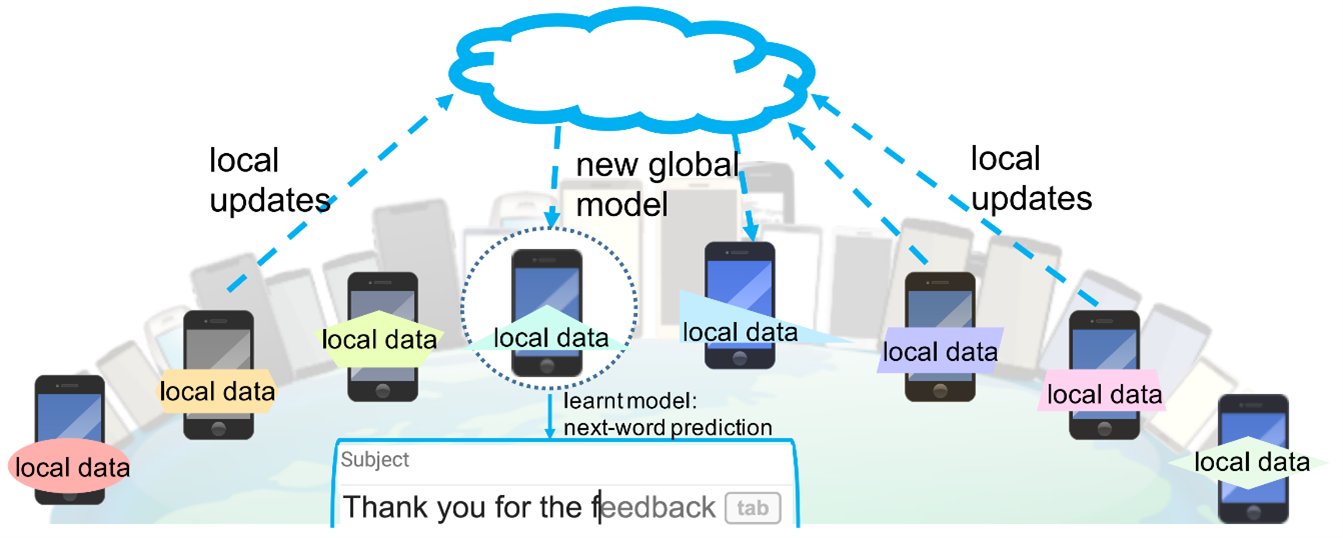
\includegraphics[scale=1]{images/chap1/gboard.png}%
	\caption{%
استفاده از یادگیری فدرال برای پیش‌بینی کلمه بعدی در
\lr{Gboard}
		\cite{li2020federated}%
		.
	}
	\label{gboard}
	\centering
\end{figure}



\section{کاربرد یادگیری فدرال}
ارتباطات نرم‌افزاری و سخت‌افزاری به معنای توانایی تبادل داده‌ها و هماهنگی عملکرد بین اجزای مختلف یک سیستم است، به طوری که این اجزا بتوانند به صورت یکپارچه و هماهنگ با یکدیگر کار کنند. فناوری مبتنی بر صنعت 4٫0%
\LTRfootnote{Industry 4.0}%
، این ارتباطات را در انواع سیستم‌ها به طور گسترده‌ای گسترش داده است. این هماهنگی بین نرم‌افزار و سخت‌افزار، به یک پدیده مهم در محیط‌های هوشمند و خودکار تبدیل شده است.

سامانه‌های متمرکز قبلی که تنها مسئول جمع‌آوری، پایش و کنترل شرایط به صورت محلی بودند، اکنون جای خود را به دستگاه‌های هوشمندی داده‌اند که قابلیت پردازش و برنامه‌ریزی داده‌ها را در سطح سیار و سیستمی دارند. علاوه بر این، گسترش ارتباطات مبتنی بر اینترنت، امکان انتقال و تبادل داده‌ها بین سیستم‌های مختلف را فراهم کرده است. این تحولات منجر به کاهش نیاز به تصمیم‌گیری متمرکز و توسعه سیستم‌های کنترل و پایش پیشرفته شده است. این ویژگی‌ها، همراه با حجم روزافزون داده‌ها، یادگیری فدرال را به یکی از بهترین روش‌ها برای توسعه سیستم‌های هوشمند تبدیل کرده است
\cite{mahtab2022algorithm}.
در ادامه، سه نمونه از کاربردهای یادگیری فدرال شرح داده خواهد شد.


\subsection{یادگیری فدرال در شهر هوشمند}
در یک شهر هوشمند%
\LTRfootnote{Smart City}%
، اطلاعات جمع‌آوری شده از حسگرهای مختلف مانند داده‌های ترافیک، مصرف انرژی، پسماند شهری و رویدادهای امنیتی، ارزش بالایی دارند و به عنوان منبعی کلیدی برای بهبود عملکرد شهر هوشمند و ارتقای کیفیت زندگی شهروندان محسوب می‌شوند. اما در کنار این مزایا، حفظ حریم شخصی و امنیت اطلاعات شهروندان نیز از اهمیت بالایی برخوردار است. یادگیری فدرال به عنوان یک رویکرد نوین که مبتنی بر حفظ حریم شخصی است، در این جا به کار گرفته می‌شود.

در یک شهر هوشمند، سازمان‌های مختلف هر کدام اطلاعات خاص خود را دارند، اما این اطلاعات به طور متقابل بر یکدیگر تأثیر می‌گذارند و می‌توانند در مدیریت بهینه شهر نقش مهمی ایفا کنند. یادگیری فدرال با حفظ حریم شخصی کاربران، این امکان را فراهم می‌کند که سازمان‌ها بدون نیاز به اشتراک‌گذاری داده‌های حساس خود با یکدیگر، از داده‌های موجود بهره‌برداری کنند و مدل‌های هوش مصنوعی و الگوریتم‌های بهبود عملکرد شهر هوشمند را توسعه دهند. به عنوان مثال، با استفاده از یادگیری فدرال می‌توان بهبود مدیریت ترافیک، بهینه‌سازی مصرف انرژی، کاهش آلودگی هوا و افزایش امنیت شهری را تحقق بخشید، در حالی که حریم شخصی شهروندان به بهترین نحو ممکن حفظ می‌شود.



%در یک شهر هوشمند%
%\LTRfootnote{Smart City}%
%، اطلاعات جمع‌آوری شده از سنسورها، دستگاه‌ها و زیرساخت‌های مختلف، از جمله ترافیک، انرژی، پسماند و امنیت، به دلیل ارزش بالایی که دارند، به عنوان منبعی مهم برای بهبود عملکرد و کیفیت زندگی شهروندان محسوب می‌شوند. اما به همراه این ارزش‌ها، حفظ حریم خصوصی و امنیت اطلاعات شهروندان نیز امری بسیار حیاتی است. یادگیری فدرال به عنوان یک رویکرد نوین و مبتنی بر حفظ حریم خصوصی، در اینجا وارد عمل می‌شود.
%
%این روش امکان پردازش داده‌های حساس مانند تصاویر، داده‌های محیطی و اطلاعات مکانی در محیط محلی و توزیع شده را فراهم می‌کند، به‌طوری‌که هر قسمت از شهر می‌تواند به صورت مستقل از سایر قسمت‌ها از این داده‌ها استفاده کند. این رویکرد امکان توسعه مدل‌های هوش مصنوعی و الگوریتم‌های بهبود عملکرد شهر هوشمند را با حفظ حریم خصوصی شهروندان فراهم می‌کند. به‌عنوان مثال، از طریق استفاده از یادگیری فدرال، می‌توان بهبود در مدیریت ترافیک، بهینه‌سازی مصرف انرژی، کاهش آلودگی هوا و افزایش امنیت شهری را به دست آورد، در حالی‌که اطلاعات شخصی شهروندان محافظت می‌شود و از نگرانی‌های حریم خصوصی جلوگیری خواهد شد.


\subsection{یادگیری فدرال در بیمارستان}
در یک بیمارستان، اطلاعات پزشکی بسیار حساس و مهم است که باید محفوظ و محرمانه نگهداری شود. اما در عین حال، استفاده از این داده‌ها برای بهبود خدمات بهداشتی و درمانی نیز بسیار ارزشمند است. در اینجا مفهوم یادگیری فدرال وارد عمل می‌شود. با استفاده از روش‌های یادگیری فدرال، بیمارستان می‌تواند از داده‌های پزشکی بیماران خود برای توسعه مدل‌هایی استفاده کند که پیش‌بینی میزان زمان بستری، بهبود در تشخیص بیماری‌ها و حتی افزایش بهره‌وری پزشکان را ایجاد می‌کنند، بدون اینکه این داده‌ها به‌طور مستقیم در اختیار یک مرکز جمع‌آوری اطلاعات واقع شوند.

به عنوان مثال، با استفاده از یادگیری فدرال، مدل‌های هوش مصنوعی می‌توانند روی داده‌های محلی بیماران بیمارستان‌ها آموزش داده شوند تا بیماری‌های مختلف را شناسایی و تشخیص دهند، و اطلاعات مربوط به درمان‌های مؤثرتر را ارائه دهند، در حالی که اطلاعات حساس بیماران محافظت می‌شود. این روش به بیمارستان‌ها امکان می‌دهد که از داده‌های بیماران خود برای بهبود خدمات بهداشتی و درمانی استفاده کنند، در حالی که رعایت مقررات مربوط به حفظ حریم خصوصی و امنیت داده‌ها را به انجام رسانده‌اند. در شکل
\ref{hospital}
یک نمونه استفاده از یادگیری فدرال در سازمان‌ها به نمایش در آمده است.


\begin{figure}[t]
	\centering
	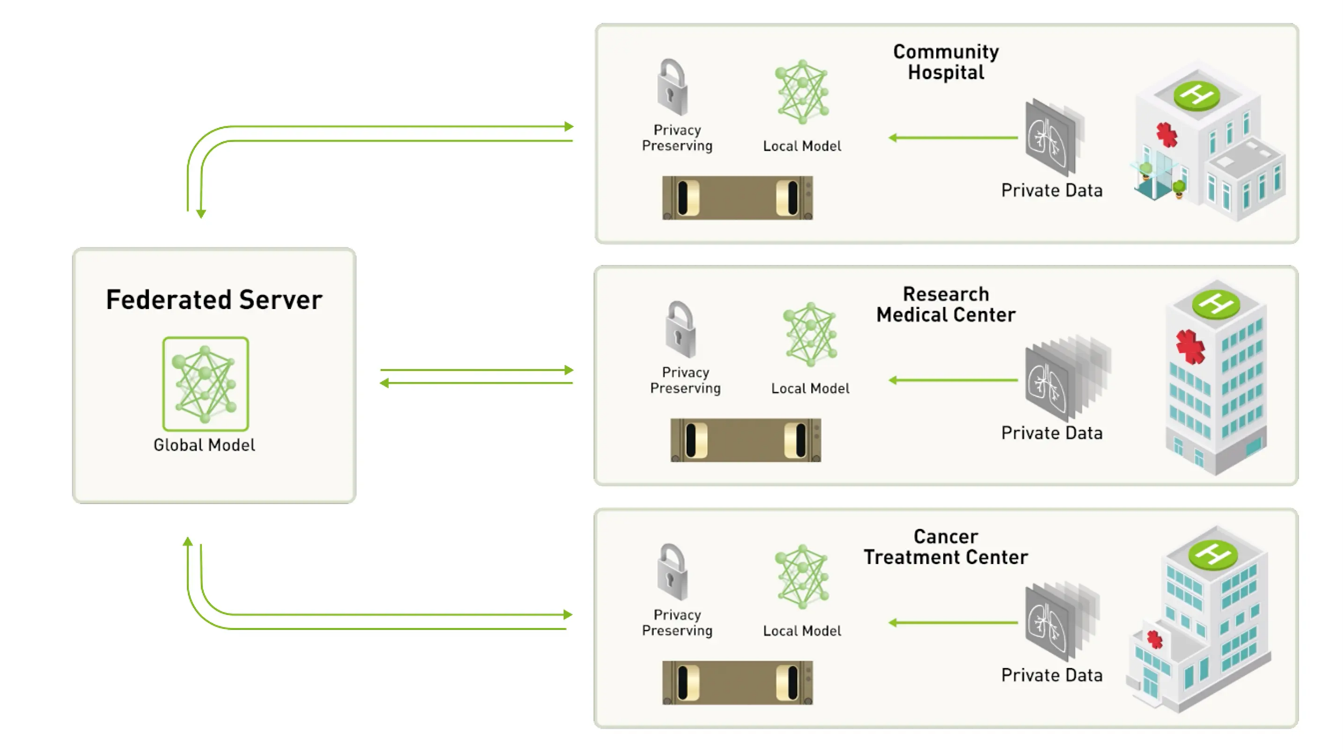
\includegraphics[scale=1]{images/chap1/hospital.png}%
	\caption{%
		یادگیری فدرال در یک بیمارستان
		\cite{kim2012control}%
		.
	}
	\label{hospital}
	\centering
\end{figure}


\subsection{یادگیری فدرال در فروشگاه برنامه‌های کاربردی موبایل}
یک فروشگاه برنامه‌های کاربردی%
\LTRfootnote{App Store}
موبایل را متصور شوید که به کاربران خود امکان می‌دهد برنامه‌های مختلف را دانلود و نصب کنند. این شرکت می‌خواهد با استفاده از داده‌های کاربران خود، الگوریتمی توسعه دهد که به طور دقیق‌تر بتواند پیشنهادات مربوط به برنامه‌هایی که کاربران ممکن است تمایل داشته باشند را ارائه کند.اگر این شرکت از روش‌های متمرکز استفاده کند، باید داده‌های حساس و شخصی کاربران را جمع‌آوری کند و برای آن‌ها تحلیل کند. این ممکن است باعث نگرانی‌های حریم خصوصی کاربران شود و از آن‌ها جلوگیری کند.

در حالی که با استفاده از یادگیری فدرال، این شرکت می‌تواند الگوریتم خود را بر روی داده‌های محلی هر تلفن هوشمند کاربر اجرا کند. به این ترتیب، هیچ داده‌ی حساسی به مرکز جمع‌آوری داده‌ها ارسال نمی‌شود و حریم خصوصی کاربران محفوظ می‌ماند. به عنوان مثال، اگر یک کاربر فقط به برنامه‌های موزیک علاقه‌مند باشد، الگوریتم محلی در تلفن هوشمند او می‌تواند این الگو را تشخیص دهد و پیشنهادات مربوط به برنامه‌های موزیک را به او ارائه دهد، بدون این‌که داده‌های شخصی و حساس او به سرور شرکت ارسال شود. این روش به شرکت امکان می‌دهد از داده‌های کاربران خود برای بهبود خدمات خود استفاده کند، در حالی که حریم خصوصی آن‌ها را محافظت می‌کند.


\section{دید کلی از روند موضوع و بیان هدف پژوهش}
تکمیل این بخش پس از رسیدن به ساختار کلی پایان‌نامه (چون ممکنه در ادامه تغییر کنه)

چند جلمه کلیدی:

به دلیل پراکندگی همگرایی به کندی صورت می‌گیرد

روش جابجایی وزن‌ها بین کاربران نهایی در طول فرایند

چرا جابجایی تصادفی، جابجایی هوشمند بر اساس میزان شباهت

\section{مروی بر روند ارائه مطالب پایان‌نامه}
تست

